% =====================================================================
%  Chapter 5 — The WIMP
% =====================================================================

\chapter{The WIMP and the Miracle That Did Not Arrive}
\label{ch:wimp}

The weakly interacting massive particle is the candidate that dark matter
research was built around for two decades. It was never observed. It remains
the most instructive of the failures in the subject, because what failed was
not the idea of a particle but the specific coupling that the idea required.

\begin{figure}[!htbp]
\centering
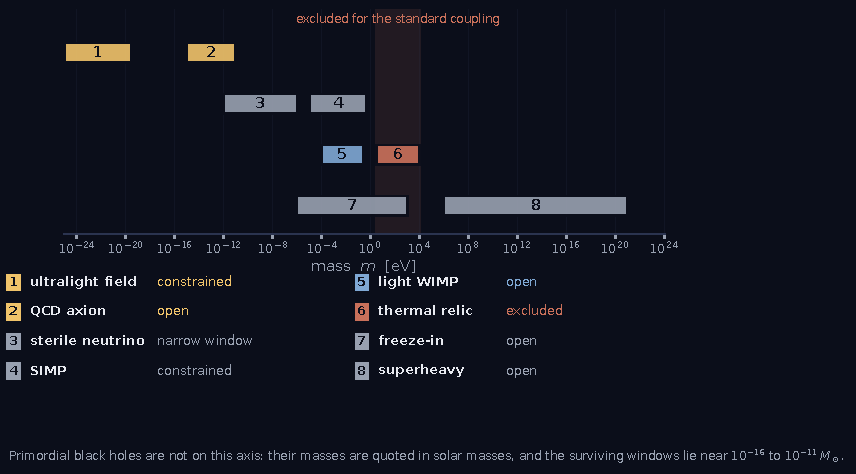
\includegraphics[width=\textwidth]{../figures/fig_candidates.pdf}
\caption{The candidate landscape on a mass axis, with the status of each class
as of late 2026. The red band marks the region in which a thermal relic with
the standard coupling is excluded; the axes are logarithmic and the figure
covers the particle candidates only, since primordial black holes are
parameterised by mass in solar masses rather than by particle mass.}
\label{fig:candidates}
\end{figure}

\figref{fig:candidates} is the map of the territory this part of the book
covers, and it is worth reading as a statement about which parts of the map
have been surveyed. The classes at the left-hand end --- the fields --- have
been constrained by cosmology and by small-scale structure. The band in the
middle is where the laboratory exclusion curves bite. The right-hand end is
where the laboratory has no leverage at all and the search for a mediator
rather than for the dark matter is the only route.

\section{The miracle}The WIMP argument is an argument about the density, not about
particle physics. Take a species with a weak-scale mass and a weak-scale
annihilation cross section, assume it was in thermal equilibrium in the early
universe, and assume it decoupled as the expansion rate outran its
interaction rate. What comes out is a relic density of order
$\Omega_\chi h^2 \sim 0.1$ --- the observed value --- with no free
parameters.

The calculation is the famous one: the annihilation rate per particle at
decoupling is roughly $3 \times 10^{-26}\ \cmthree\s$, and the resulting
density is the density we observe. There is no scale in the calculation that
was chosen; the weak scale is the weak scale, and the observed density is
what falls out.

That is what made it a miracle rather than a fit, and it is the reason the
WIMP was for decades the default answer to the question of what dark matter
is.

\section{Why it did not arrive}Two decades of dedicated experiments have now excluded
essentially all of the parameter space in which the miracle works and the
coupling is of the standard weak strength.

The current frontier is set by three tonne-scale liquid-xenon experiments.
LZ's 4.2 tonne-year exposure excludes spin-independent nucleon cross
sections above $2.2 \times 10^{-48}\ \cmtwo$ at a mass of 40~GeV
\idx{LZ Collaboration}. XENONnT's 3.1 tonne-year result reaches
$1.7 \times 10^{-47}\ \cmtwo$ at 30~GeV \idx{XENON Collaboration}, and
PandaX-4T has reached 1.54 tonne-year \idx{PandaX Collaboration}. Spin-dependent
couplings to protons are excluded to a depth of roughly $10^{-41}\ \cmtwo$
at the same masses.

Those are extraordinary numbers, and their consequence is equally
extraordinary in its way: the region of the classic parameter space where a
thermal relic with a weak-scale cross section would be found is gone. The
minimal supersymmetric model, the most natural home for a WIMP, has been
closed in most of its parameter space by a combination of these searches, the
LEP and LHC bounds, and the measured relic density.

\section{What survives, and why the word ``WIMP'' has drifted}Three things survive, and it matters that they are
different things.

The first is \emph{the miracle itself}. The statement that a thermal relic
of weak-scale mass with a weak-scale cross section reproduces the observed
density remains true, and it remains unexplained by anything else. The
coincidence has not been dissolved; it has been moved.

The second is \emph{the candidate class}. A weakly interacting massive
particle is still entirely viable if any of its three assumptions changes:
if the thermal history was different, if the interaction is weaker than the
standard weak strength, or if the mass is much lighter or much heavier than
the electroweak scale. Most of the surviving parameter space lives in these
regions.

The third is \emph{a specific and fertile corner}: the coannihilation
regime, in which a subdominant species annihilates efficiently with the
dominant one, and the resonance regime, in which annihilation proceeds
through a near-threshold particle on shell. Both mechanisms can produce the
observed density while suppressing the direct-detection rate, and both are
constrained by a combination of relic density, collider bounds and direct
detection that no single experiment controls.

The terminological drift matters for reading the literature. ``WIMP'' is
used for the weak-scale thermal relic, for the weakly interacting massive
particle in general, and sometimes loosely for any particle with weak-scale
interactions. The exclusion plots are drawn against the third usage; the
miracle belongs to the first.

\section{The failure modes of the idea}Three specific failures have been diagnosed, and each
teaches something that applies beyond the WIMP.

The \emph{coannihilation and resonance mechanisms} fail in the sense that
they are not predictions: they work for a broad range of masses and
couplings, and the particle content required to make them work is
uncomfortably large.

The \emph{flat or sphaleron-mediated direction} --- in which the dark sector
communicates with the Standard Model through an electroweak instanton ---
leads to wrong-flavour and is essentially excluded by flavour physics.

The \emph{asymmetric dark matter} scenario --- in which the relic abundance
is the excess of particles over antiparticles, and the annihilation rate
today can be arbitrarily small --- survives direct detection comfortably, and
it pays for that by giving up the explanation of the density.

\section{What would settle it}A WIMP would be confirmed by a nuclear recoil above the
neutrino floor with the recoil spectrum of elastic scattering, seen by two
experiments with different targets and different systematics, at a
cross section and mass that the current nulls exclude. A null does not
exclude the class, because the class has moved. But the current exclusion
region should not be searched again with more of the same detector.

\begin{keytakeaways}
\item The WIMP miracle is a statement about the relic density, and it
remains unexplained; what was excluded is the specific combination of
weak-scale mass and weak-scale coupling.
\item The classic parameter space is closed. The surviving WIMP-like region
lives in modified thermal histories, suppressed couplings, and the
coannihilation and resonance corners.
\item ``WIMP'' means three different things in the literature, and the
exclusion curves apply to only one of them.
\item The failure was not of the idea of a particle dark matter but of its
standard coupling, which is the more useful lesson.
\end{keytakeaways}
